\chapter{Analysis of \texorpdfstring{$2\nu\boldsymbol{\beta}\boldsymbol{\beta}$}{2nu beta beta} data}
\label{chapter:2nubb-data}
The latest step of this analysis involves testing all the deep learning models discussed so far with data that are well-known \ac{SSE}-like events.

\begin{figure}[H]
    \centering
    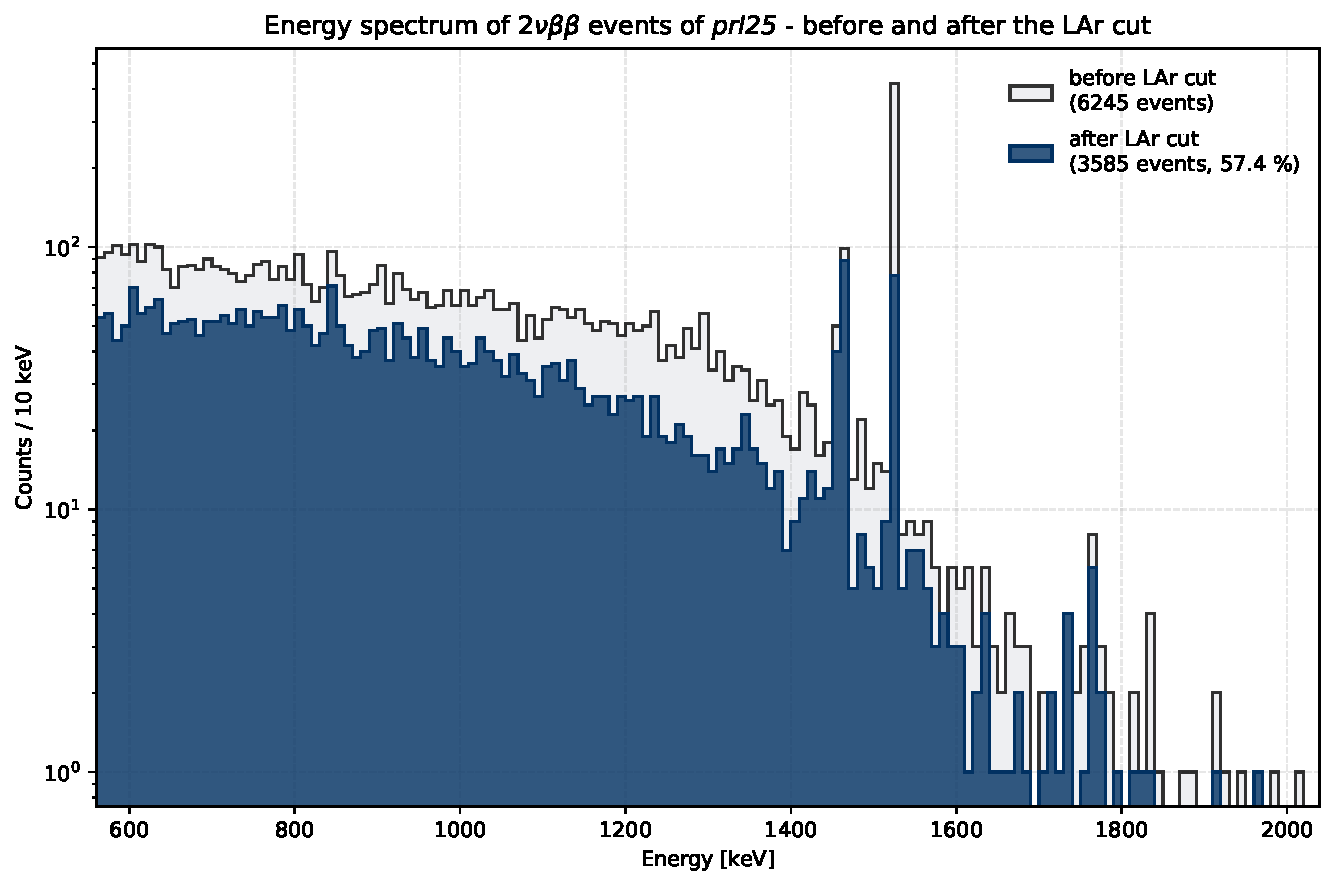
\includegraphics[width=0.8\textwidth]{plots/2nubb/energy_spectrum_before_after_LAr.pdf}
    \caption{Energy spectrum of the $2\nu\beta\beta$ data before (grey) and after (blue) the \ac{lar} cut.}
    \label{fig:2nu-beforeafterLAR}
\end{figure}

\begin{figure}[H]
    \centering
    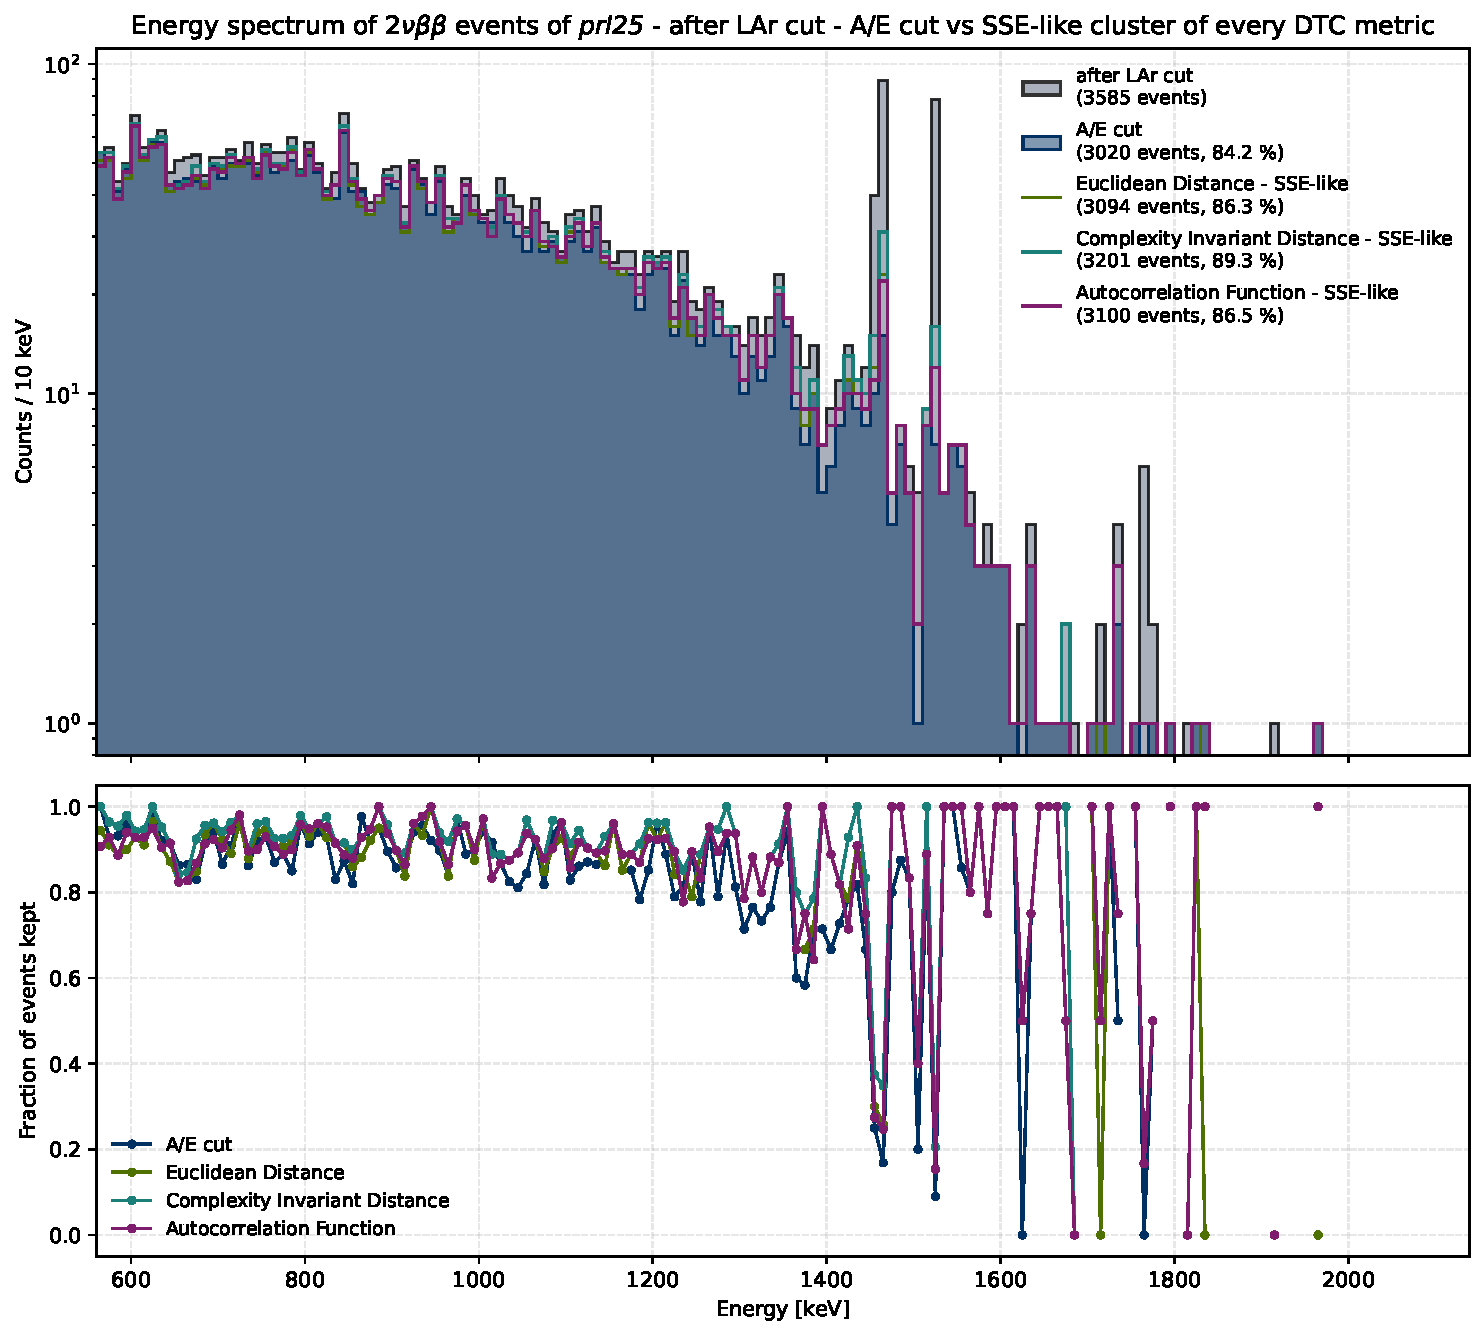
\includegraphics[width=0.8\textwidth]{plots/2nubb/energy_spectrum_AoE_vs_DTC_afterLAr.pdf}
    \caption{Energy spectrum of the $2\nu\beta\beta$ data with different \ac{PSD} cuts: standard \ac{AE} cut and different \ac{DTC} metrics cuts.}
    \label{fig:2nu-AEandDTCcuts}
\end{figure}

\begin{figure}[H]
    \centering
    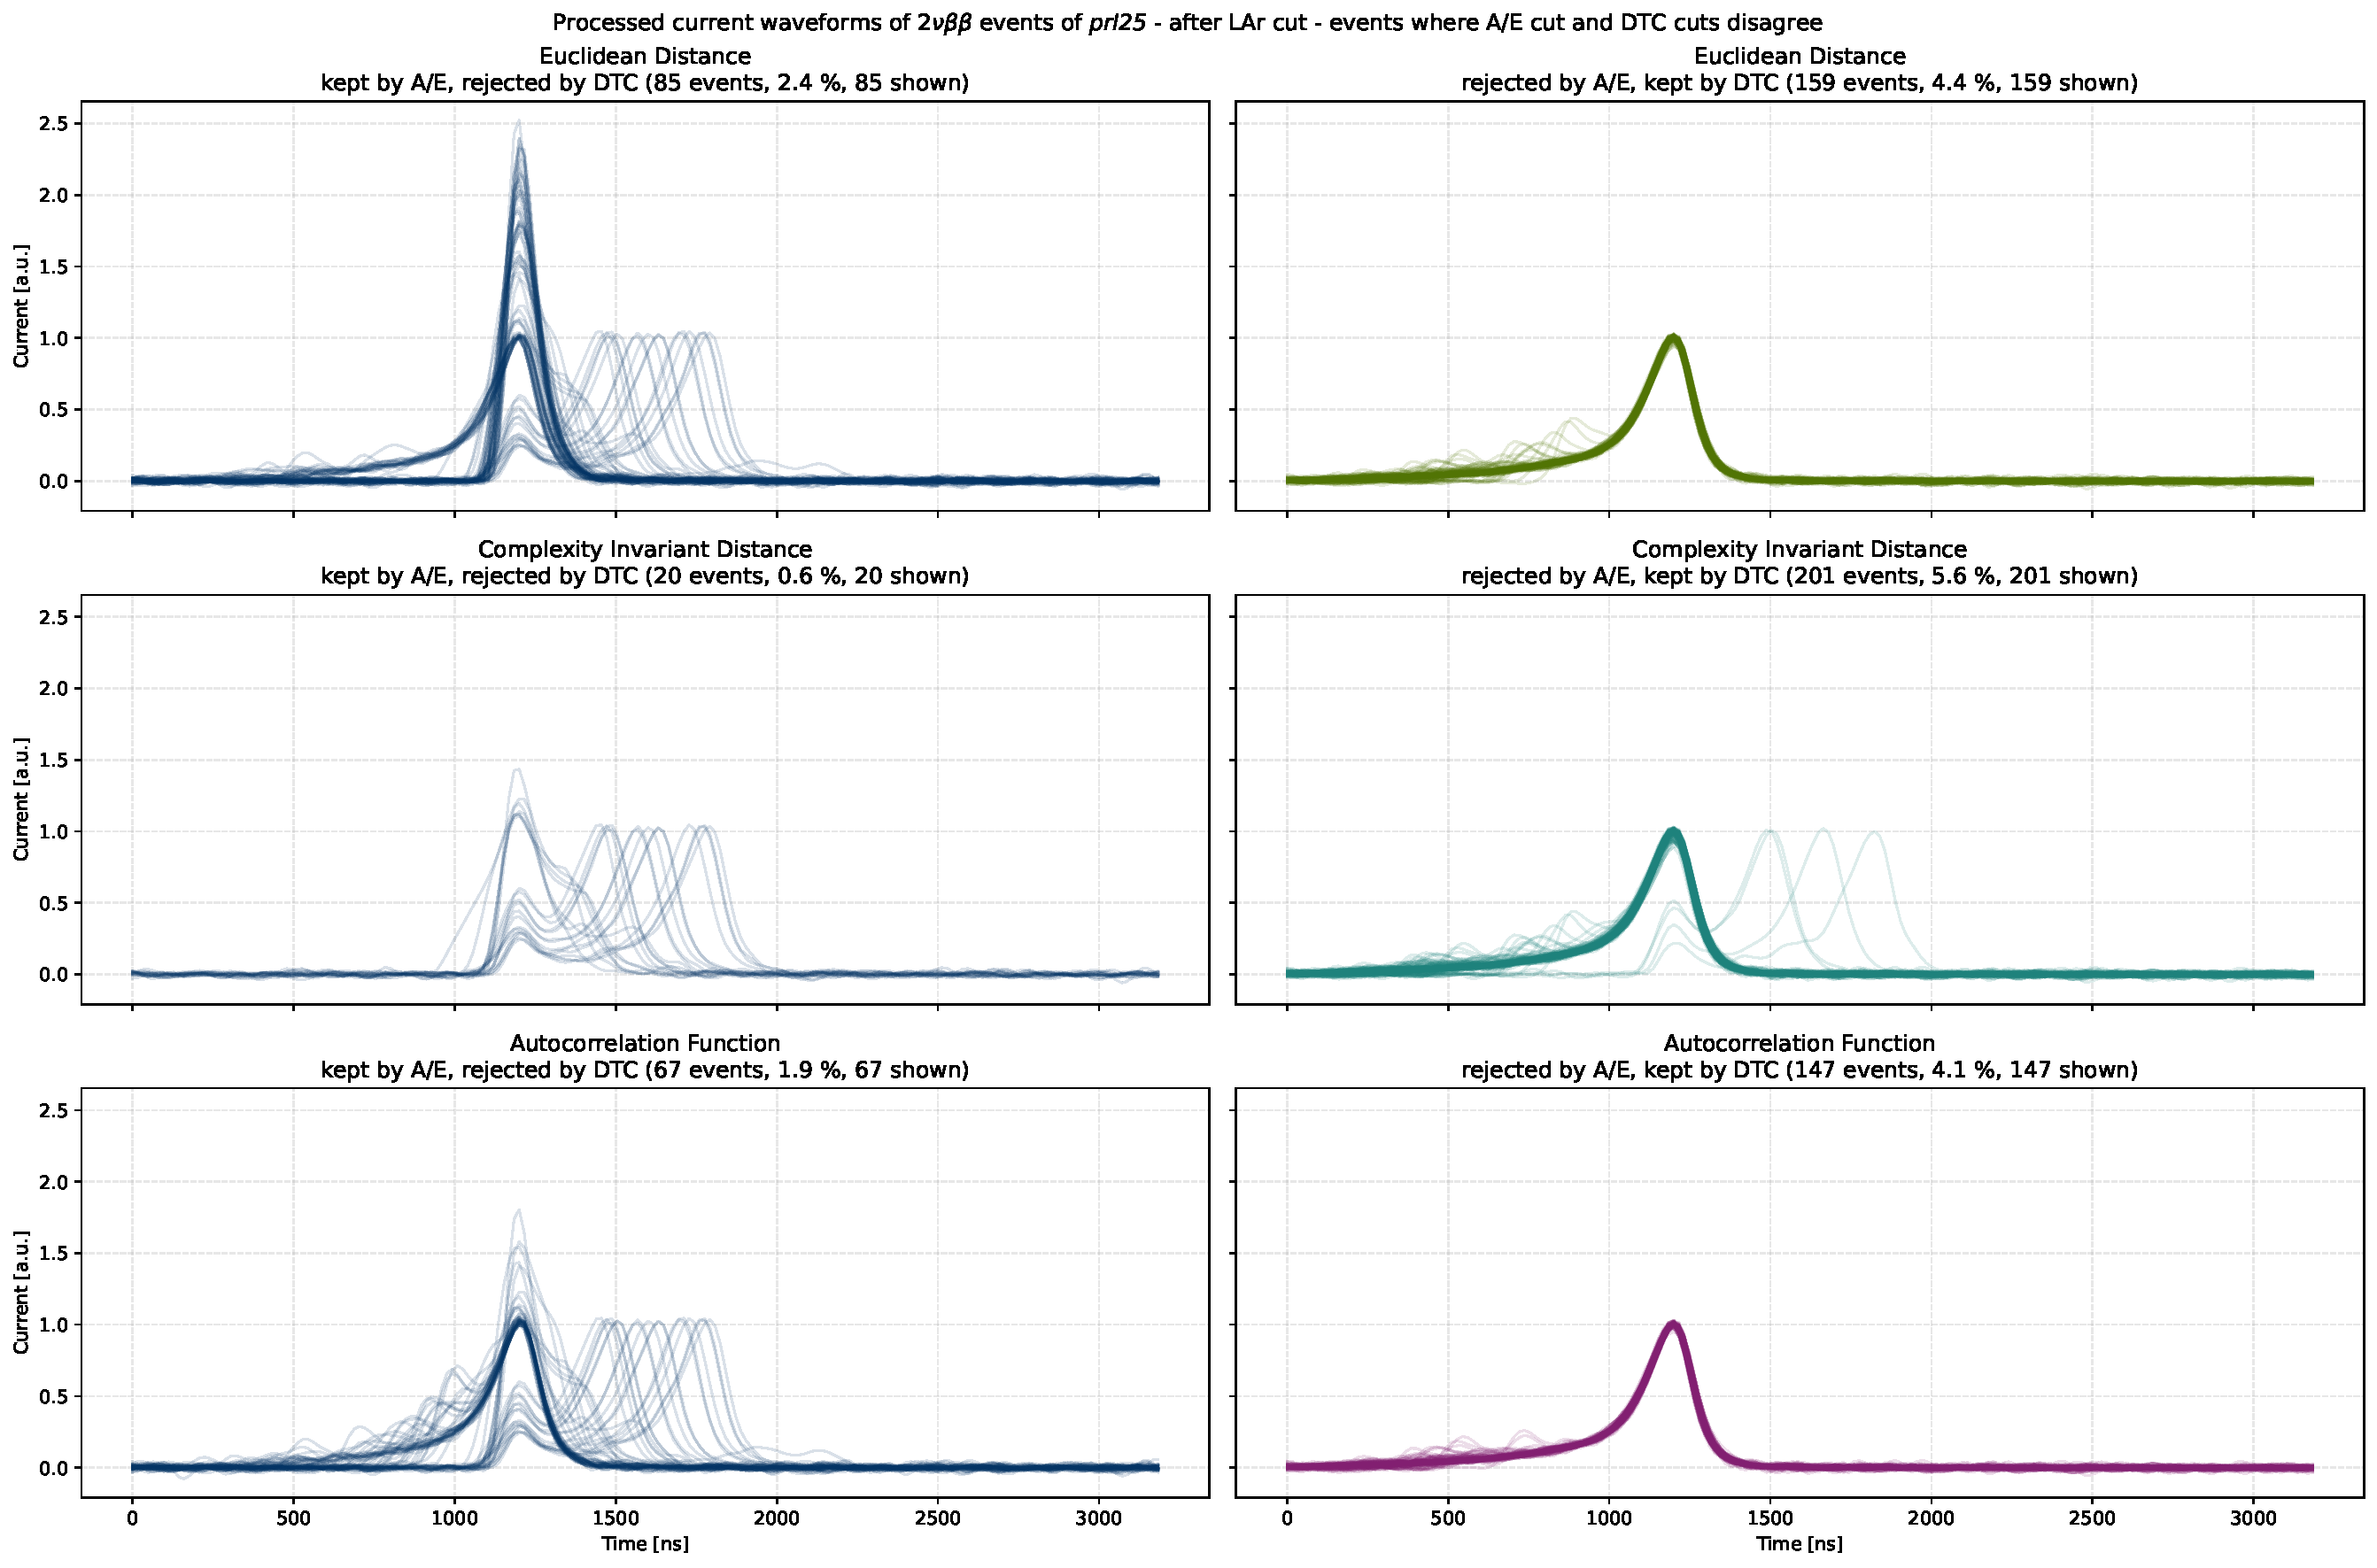
\includegraphics[width=\textwidth]{plots/2nubb/waveforms_AoE_DTC_disagree_afterLAr.pdf}
    \caption{Comparison between current waveforms kept and rejectd by different cuts: On th eleft waveforms kept by the \ac{AE} cuts but rejected by a specific \ac{DTC} metric cut, viceversa on the right events rejected by the \ac{DTC} metric but kept by \ac{AE} are shown. From the top to the bottom Euclidean Distance, Complexity Invariant Distance and Autocorrelation Function.}
    \label{fig:2nu-kept_rejected_AE_DTC}
\end{figure}